% --- shared colours (matplotlib tab10) ---
\definecolor{cblue}{RGB}{31,119,180}
\definecolor{cred}{RGB}{214,39,40}
\definecolor{cgreen}{RGB}{44,160,44}

% common picture options: 1 bit = 0.042 cm on both axes (square aspect)
\tikzset{bitsec/.style={x=0.042cm,y=0.042cm,font=\small}}

%======================================================================
% PANEL 1a:  Additive loss, linear attack
%======================================================================
\newcommand{\panelAddLin}{%
  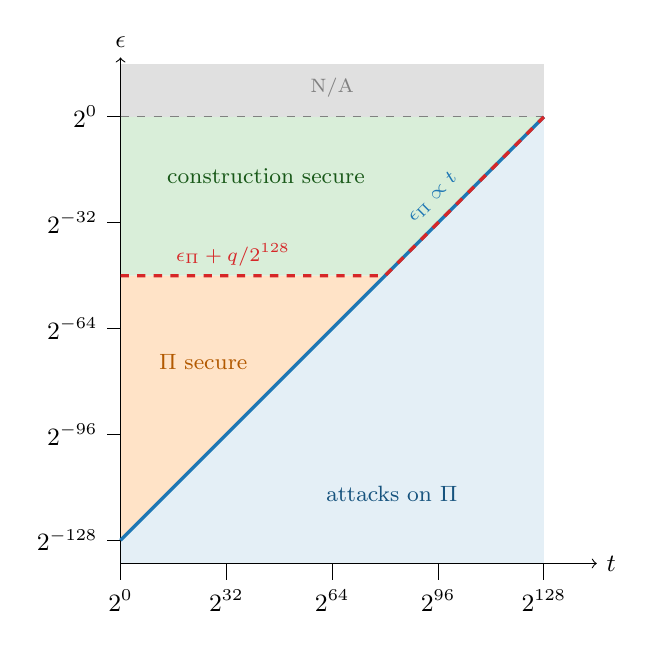
\begin{tikzpicture}[bitsec]
    \def\n{128}
    \fill[black!12]  (0,0) -- (0,16) -- (\n,16) -- (\n,0) -- cycle;
    \fill[cblue!12]  (0,-\n) -- (\n,0) -- (\n,-135) -- (0,-135) -- cycle;
    \fill[orange!22] (0,-\n) -- (0,-48) -- (80,-48) -- cycle;                 % gap
    \fill[cgreen!18] (0,0) -- (0,-48) -- (80,-48) -- (\n,0) -- cycle;          % construction secure
    \draw[->] (0,-135) -- (0,18) node[above] {$\epsilon$};
    \draw[->] (0,-135) -- ({\n+16},-135) node[right] {$t$};
    \foreach \x in {0,32,64,96,128} \draw (\x,-135)--(\x,-140) node[below] {$2^{\x}$};
    \foreach \y in {0,-32,-64,-96,-128} \draw (0,\y)--(-4,\y) node[left] {$2^{\y}$};
    \draw[gray,dashed] (0,0) -- (\n,0);
    \node[gray,font=\scriptsize] at ({0.5*\n},9) {N/A};
    \draw[cblue,very thick] (0,-\n) -- (\n,0);
    \draw[cred,very thick,dashed] (0,-48) -- (80,-48) -- (\n,0);
    \node[cblue,rotate=45,anchor=south,font=\scriptsize] at (98,-28) {$\epsilon_\Pi \propto t$};
    \node[cred,anchor=south,font=\scriptsize] at (34,-48) {$\epsilon_\Pi + q/2^{128}$};
    \node[cgreen!55!black,align=center,font=\footnotesize] at (44,-18) {construction secure};
    \node[orange!70!black,align=center,font=\footnotesize] at (25,-74) {$\Pi$ secure};
    \node[cblue!70!black,align=center,font=\footnotesize] at (82,-114) {attacks on $\Pi$};
  \end{tikzpicture}
}

%======================================================================
% PANEL 1b:  Additive loss, quadratic attack
%======================================================================
\newcommand{\panelAddQuad}{%
  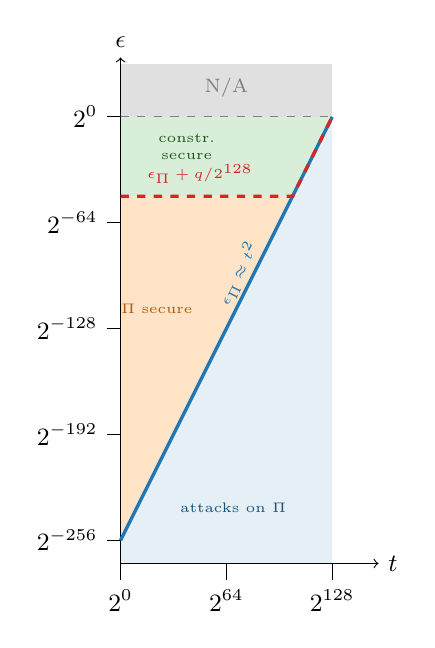
\begin{tikzpicture}[bitsec]
    \def\n{128}\def\m{64}
    \fill[black!12]  (0,0) -- (0,16) -- (\m,16) -- (\m,0) -- cycle;
    \fill[cblue!12]  (0,-\n) -- (\m,0) -- (\m,-135) -- (0,-135) -- cycle;
    \fill[orange!22] (0,-24) -- (52,-24) -- (0,-\n) -- cycle;
    \fill[cgreen!18] (0,0) -- (0,-24) -- (52,-24) -- (\m,0) -- cycle;
    \draw[->] (0,-135) -- (0,18) node[above] {$\epsilon$};
    \draw[->] (0,-135) -- ({\m+14},-135) node[right] {$t$};
    \foreach \x in {0,64,128} \draw ({\x/2},-135)--({\x/2},-140) node[below] {$2^{\x}$};
    \foreach \y in {0,-64,-128,-192,-256} \draw (0,{\y/2})--(-4,{\y/2}) node[left] {$2^{\y}$};
    \draw[gray,dashed] (0,0) -- (\m,0);
    \node[gray,font=\scriptsize] at (32,9) {N/A};
    \draw[cblue,very thick] (0,-\n) -- (\m,0);
    \draw[cred,very thick,dashed] (0,-24) -- (52,-24) -- (\m,0);
    \node[cblue,rotate=63.43,anchor=south,font=\tiny] at (41,-50) {$\epsilon_\Pi \approx t^2$};
    \node[cred,anchor=south,font=\tiny] at (24,-23) {$\epsilon_\Pi + q/2^{128}$};
    \node[cgreen!55!black,align=center,font=\tiny] at (20,-9) {constr.\\secure};
    \node[orange!70!black,align=center,font=\tiny] at (11,-58) {$\Pi$ secure};
    \node[cblue!70!black,align=center,font=\tiny] at (34,-118) {attacks on $\Pi$};
  \end{tikzpicture}
}

%======================================================================
% PANEL 1c:  Additive loss, cubic attack
%======================================================================
\newcommand{\panelAddCube}{%
  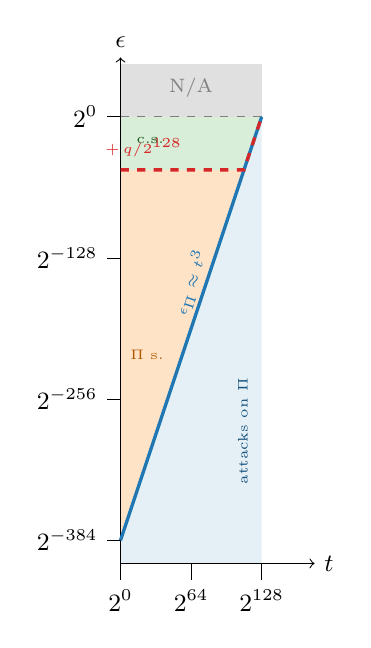
\begin{tikzpicture}[bitsec]
    \def\n{128}
    \fill[black!12]  (0,0) -- (0,16) -- ({\n/3},16) -- ({\n/3},0) -- cycle;
    \fill[cblue!12]  (0,-\n) -- ({\n/3},0) -- ({\n/3},-135) -- (0,-135) -- cycle;
    \fill[orange!22] (0,-16) -- (37.333,-16) -- (0,-\n) -- cycle;
    \fill[cgreen!18] (0,0) -- (0,-16) -- (37.333,-16) -- ({\n/3},0) -- cycle;
    \draw[->] (0,-135) -- (0,18) node[above] {$\epsilon$};
    \draw[->] (0,-135) -- ({\n/3+16},-135) node[right] {$t$};
    \foreach \x in {0,64,128} \draw ({\x/3},-135)--({\x/3},-140) node[below] {$2^{\x}$};
    \foreach \y in {0,-128,-256,-384} \draw (0,{\y/3})--(-4,{\y/3}) node[left] {$2^{\y}$};
    \draw[gray,dashed] (0,0) -- ({\n/3},0);
    \node[gray,font=\scriptsize] at ({\n/6},9) {N/A};
    \draw[cblue,very thick] (0,-\n) -- ({\n/3},0);
    \draw[cred,very thick,dashed] (0,-16) -- (37.333,-16) -- ({\n/3},0);
    \node[cblue,rotate=71.57,anchor=south,font=\tiny] at (27,-52) {$\epsilon_\Pi \approx t^3$};
    \node[cred,anchor=south,font=\tiny] at (7,-15) {$+\,q/2^{128}$};
    \node[cgreen!55!black,align=center,font=\tiny] at (9,-7) {c.s.};
    \node[orange!70!black,align=center,font=\tiny] at (8,-72) {$\Pi$ s.};
    \node[cblue!70!black,align=center,font=\tiny,rotate=90] at (37,-95) {attacks on $\Pi$};
  \end{tikzpicture}
}

%======================================================================
% PANEL 2a:  Multiplicative loss, linear attack
%======================================================================
\newcommand{\panelMultLin}{%
  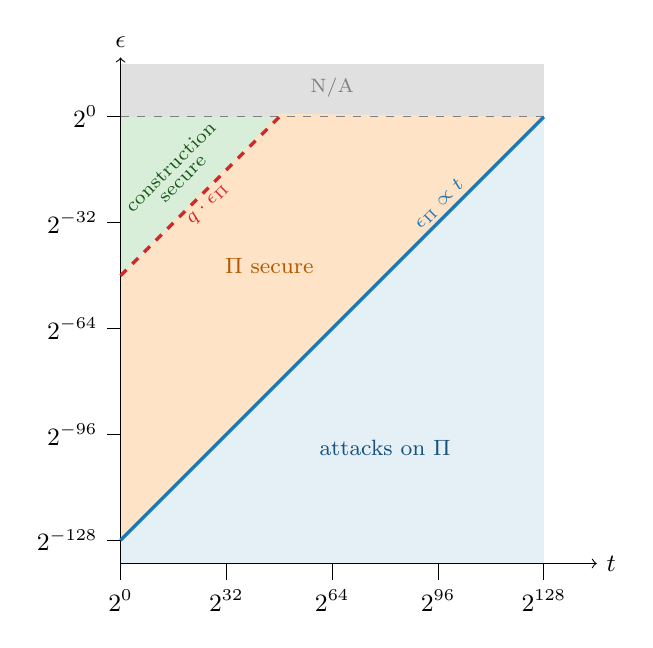
\begin{tikzpicture}[bitsec]
    \def\n{128}\def\l{80}
    \fill[black!12]   (0,0) -- (0,16) -- (\n,16) -- (\n,0) -- cycle;
    \fill[cgreen!18] (0,{-\n+\l}) -- (0,0) -- ({\n-\l},0) -- cycle;
    \fill[orange!22] (0,{-\n}) -- (0,{-\n+\l}) -- ({\n-\l},) -- (\n,0) -- cycle;
    \fill[cblue!12]  (0,-\n) -- (\n,0) -- (\n,-135) -- (0,-135) -- cycle;
    \draw[->] (0,-135) -- ({\n+16},-135) node[right] {$t$}; % x-axis
    \draw[->] (0,-135) -- (0,18) node[above] {$\epsilon$}; % y-axis
    \foreach \x in {0,32,64,96,128} \draw (\x,-135)--(\x,-140) node[below] {$2^{\x}$}; % x-axis labels
    \foreach \y in {0,-32,-64,-96,-128} \draw (0,\y)--(-4,\y) node[left] {$2^{\y}$}; % y-axis labes
    %\node[gray,rotate=90,anchor=south,font=\scriptsize] at (-24,-68) {$\downarrow$ more secure};
    \draw[gray,dashed] (0,0) -- (\n,0); % gray top line
    \node[gray,font=\scriptsize] at ({0.5*\n},9) {N/A}; % top line legend
    \draw[cred,very thick,dashed] (0,{-\n+\l}) -- ({\n-\l},0); % red middle line
    \draw[cblue,very thick] (0,-\n) -- (\n,0); % blue bottom line
    \node[cblue,rotate=45,anchor=south,font=\scriptsize] at (100,-30) {$\epsilon_\Pi \propto t$};
    \node[cred,rotate=45,anchor=south,font=\scriptsize] at (30,-30) {$q \cdot \epsilon_\Pi$};
    \node[cgreen!55!black,align=center,rotate=45,font=\scriptsize] at (15,-15) 
      {construction};
    \node[cgreen!55!black,align=center,rotate=45,font=\scriptsize] at (19,-19) 
      {secure};
    \node[orange!70!black,align=center,font=\footnotesize] at (45,-45)
      %{primitive secure \\ construction broken?};
      {$\Pi$ secure};
    \node[cblue!70!black,align=center,font=\footnotesize] at (80,-100) 
      {attacks on $\Pi$};
  \end{tikzpicture}
}

%======================================================================
% PANEL 2b:  Multiplicative loss, quadratic attack
%======================================================================
\newcommand{\panelMultQuad}{%
  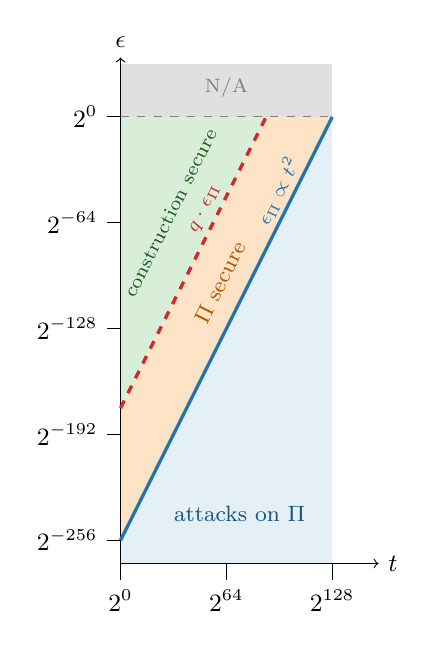
\begin{tikzpicture}[bitsec]
    \def\n{128}\def\m{64}\def\l{40} % everything scaled by x2 
    \fill[black!12]   (0,0) -- (0,16) -- (\m,16) -- (\m,0) -- cycle;
    \fill[cgreen!18] (0,{-\n+\l}) -- (0,0) -- ({(\n-\l)/2},0) -- cycle;
    \fill[orange!22] (0,{-\n+\l}) -- (0,{-\n}) -- (\m,0) -- ({(\n-\l)/2},0) -- cycle;
    \fill[cblue!12]  (0,-\n) -- (\m,0) -- (\m,-135) -- (0,-135) -- cycle;
    \draw[->] (0,-135) -- (0,18) node[above] {$\epsilon$};
    \draw[->] (0,-135) -- ({\m+14},-135) node[right] {$t$};
    \foreach \x in {0,64,128} \draw ({\x/2},-135)--({\x/2},-140) node[below] {$2^{\x}$};
    \foreach \y in {0,-64,-128,-192,-256} \draw (0,{\y/2})--(-4,{\y/2}) node[left] {$2^{\y}$};
    \draw[gray,dashed] (0,0) -- (\m,0);
    \node[gray,font=\scriptsize] at (32,9) {N/A};
    \draw[cred,very thick,dashed] (0,{-\n+\l}) -- ({(\n-\l)/2},0);
    \draw[cblue,very thick] (0,-\n) -- (\m,0);
    \node[cblue,rotate=63.43,anchor=south,font=\scriptsize] at (53,-25) {$\epsilon_\Pi \propto t^2$};
    \node[cred,rotate=63.43,anchor=south,font=\scriptsize] at (30,-30) {$q\cdot\epsilon_\Pi$};
    \node[cgreen!55!black,align=center,rotate=63.43,font=\scriptsize] at (15,-29) 
      {construction secure};
    \node[orange!70!black,align=center,rotate=63.43,font=\footnotesize] at (30,-50)
      %{primitive secure \\ construction broken?};
      {$\Pi$ secure};
    \node[cblue!70!black,align=center,font=\footnotesize] at (36,-120) 
      {attacks on $\Pi$};
  \end{tikzpicture}
}

%======================================================================
% PANEL 2c:  Multiplicative loss, cubic attack
%======================================================================
\newcommand{\panelMultCube}{%
  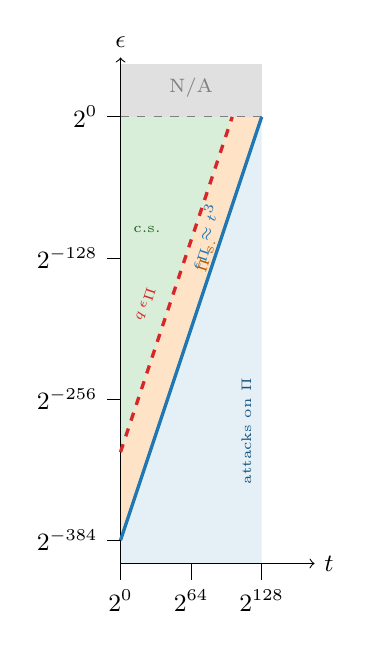
\begin{tikzpicture}[bitsec]
    \def\n{128}
    \fill[black!12]  (0,0) -- (0,16) -- ({\n/3},16) -- ({\n/3},0) -- cycle;
    \fill[cblue!12]  (0,-\n) -- ({\n/3},0) -- ({\n/3},-135) -- (0,-135) -- cycle;
    \fill[orange!22] (0,-\n) -- ({\n/3},0) -- (33.778,0) -- (0,-101.333) -- cycle;
    \fill[cgreen!18] (0,0) -- (0,-101.333) -- (33.778,0) -- cycle;
    \draw[->] (0,-135) -- (0,18) node[above] {$\epsilon$};
    \draw[->] (0,-135) -- ({\n/3+16},-135) node[right] {$t$};
    \foreach \x in {0,64,128} \draw ({\x/3},-135)--({\x/3},-140) node[below] {$2^{\x}$};
    \foreach \y in {0,-128,-256,-384} \draw (0,{\y/3})--(-4,{\y/3}) node[left] {$2^{\y}$};
    \draw[gray,dashed] (0,0) -- ({\n/3},0);
    \node[gray,font=\scriptsize] at ({\n/6},9) {N/A};
    \draw[cblue,very thick] (0,-\n) -- ({\n/3},0);
    \draw[cred,very thick,dashed] (0,-101.333) -- (33.778,0);
    \node[cblue,rotate=71.57,anchor=south,font=\tiny] at (31,-38) {$\epsilon_\Pi \approx t^3$};
    \node[cred,rotate=71.57,anchor=south,font=\tiny] at (12,-58) {$q\,\epsilon_\Pi$};
    \node[cgreen!55!black,align=center,font=\tiny] at (8,-34) {c.s.};
    \node[orange!70!black,align=center,font=\tiny,rotate=71.57] at (26,-42) {$\Pi$ s.};
    \node[cblue!70!black,align=center,font=\tiny,rotate=90] at (38,-95) {attacks on $\Pi$};
  \end{tikzpicture}
}

%======================================================================
% PANEL 3a:  Square-root loss, linear attack
%======================================================================
\newcommand{\panelRootLin}{%
  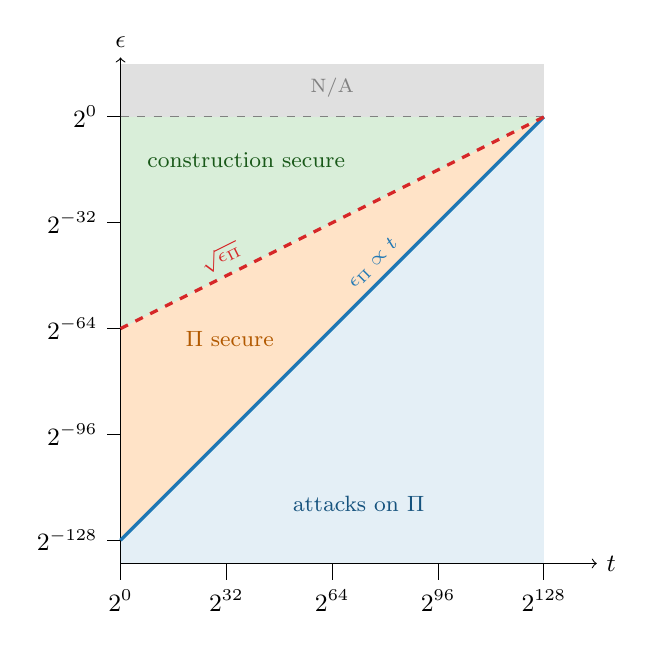
\begin{tikzpicture}[bitsec]
    \def\n{128}
    \fill[black!12]   (0,0) -- (0,16) -- (\n,16) -- (\n,0) -- cycle;
    \fill[cblue!12]  (0,-\n) -- (\n,0) -- (\n,-135) -- (0,-135) -- cycle;
    \fill[orange!22] (0,-\n) -- (0,{-\n/2}) -- (\n,0) -- cycle;
    \fill[cgreen!18] (0,{-\n/2}) -- (0,0) -- (\n,0) -- cycle;
    \draw[->] (0,-135) -- (0,18) node[above] {$\epsilon$};
    \draw[->] (0,-135) -- ({\n+16},-135) node[right] {$t$};
    \foreach \x in {0,32,64,96,128} \draw (\x,-135)--(\x,-140) node[below] {$2^{\x}$};
    \foreach \y in {0,-32,-64,-96,-128} \draw (0,\y)--(-4,\y) node[left] {$2^{\y}$};
    %\node[gray,rotate=90,anchor=south,font=\scriptsize] at (-24,-68) {$\downarrow$ more secure};
    \draw[gray,dashed] (0,0) -- (\n,0);
    \node[gray,font=\scriptsize] at ({0.5*\n},9) {N/A};
    \draw[cblue,very thick] (0,-\n) -- (\n,0);
    \draw[cred,very thick,dashed] (0,{-\n/2}) -- (\n,0);
    \node[cblue,rotate=45,anchor=south,font=\scriptsize] at (80,-48) {$\epsilon_\Pi \propto t$};
    \node[cred,rotate=26.57,anchor=south,font=\scriptsize] at (33,-48) {$\sqrt{\epsilon_\Pi}$};
    \node[cgreen!55!black,align=center,font=\footnotesize] at (38,-13) 
      {construction secure};
    \node[orange!70!black,align=center,font=\footnotesize] at (33,-67)
      %{primitive secure \\ construction broken?};
      {$\Pi$ secure};
    \node[cblue!70!black,align=center,font=\footnotesize] at (72,-117) 
      {attacks on $\Pi$};
  \end{tikzpicture}
}

%======================================================================
% PANEL 3b:  Square-root loss, quadratic attack
%======================================================================
\newcommand{\panelRootQuad}{%
  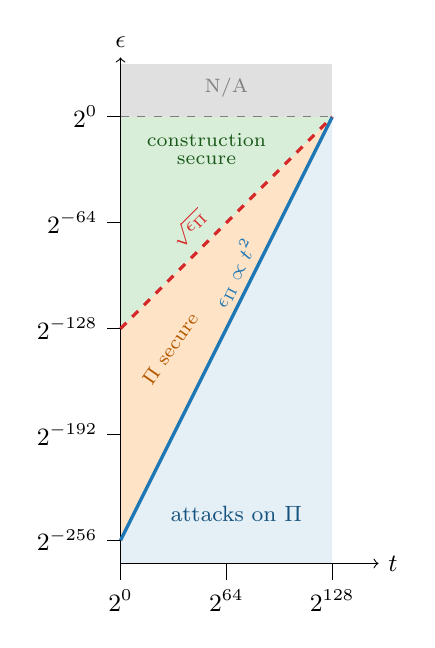
\begin{tikzpicture}[bitsec]
    \def\n{128}\def\m{64}
    \fill[black!12]   (0,0) -- (0,16) -- (\m,16) -- (\m,0) -- cycle;
    \fill[cblue!12]  (0,-\n) -- (\m,0) -- (\m,-135) -- (0,-135) -- cycle;
    \fill[orange!22] (0,-\n) -- (0,-\m) -- (\m,0) -- cycle;
    \fill[cgreen!18] (0,-\m) -- (0,0) -- (\m,0) -- cycle;
    \draw[->] (0,-135) -- (0,18) node[above] {$\epsilon$};
    \draw[->] (0,-135) -- ({\m+14},-135) node[right] {$t$};
    \foreach \x in {0,64,128} \draw ({\x/2},-135)--({\x/2},-140) node[below] {$2^{\x}$};
    \foreach \y in {0,-64,-128,-192,-256} \draw (0,{\y/2})--(-4,{\y/2}) node[left] {$2^{\y}$};
    \draw[gray,dashed] (0,0) -- (\m,0);
    \node[gray,font=\scriptsize] at (32,9) {N/A};
    \draw[cblue,very thick] (0,-\n) -- (\m,0);
    \draw[cred,very thick,dashed] (0,-\m) -- (\m,0);
    \node[cblue,rotate=63.43,anchor=south,font=\scriptsize] at (40,-50) {$\epsilon_\Pi \propto t^2$};
    \node[cred,rotate=45,anchor=south,font=\scriptsize] at (25,-38) {$\sqrt{\epsilon_\Pi}$};
    \node[cgreen!55!black,align=center,font=\scriptsize] at (26,-7) {construction};
    \node[cgreen!55!black,align=center,font=\scriptsize] at (26,-13) {secure};
    \node[orange!70!black,align=center,rotate=55,font=\scriptsize] at (15,-70) {$\Pi$ secure};
    \node[cblue!70!black,align=center,font=\footnotesize] at (35,-120) {attacks on $\Pi$};
  \end{tikzpicture}
}

%======================================================================
% PANEL 3c:  Square-root loss, qubic attack
%======================================================================
\newcommand{\panelRootCube}{%
  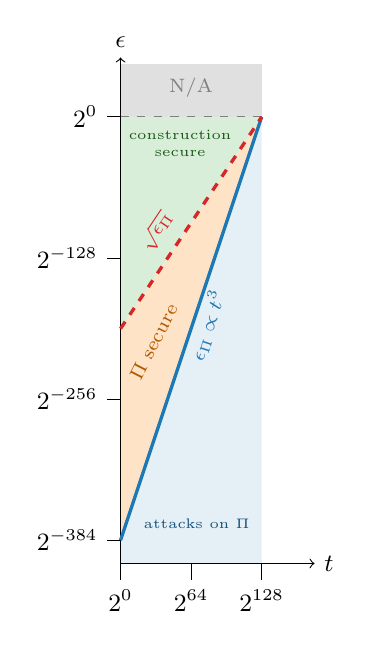
\begin{tikzpicture}[bitsec]
    \def\n{128}% depth 128 drawn = 384 bits; pinch x = \n/3
    \fill[black!12]  (0,0) -- (0,16) -- ({\n/3},16) -- ({\n/3},0) -- cycle;
    \fill[cblue!12]  (0,-\n) -- ({\n/3},0) -- ({\n/3},-135) -- (0,-135) -- cycle;
    \fill[orange!22] (0,-\n) -- (0,{-\n/2}) -- ({\n/3},0) -- cycle;
    \fill[cgreen!18] (0,{-\n/2}) -- (0,0) -- ({\n/3},0) -- cycle;
    \draw[->] (0,-135) -- (0,18) node[above] {$\epsilon$};
    \draw[->] (0,-135) -- ({\n/3+16},-135) node[right] {$t$};
    \foreach \x in {0,64,128} \draw ({\x/3},-135)--({\x/3},-140) node[below] {$2^{\x}$};
    \foreach \y in {0,-128,-256,-384} \draw (0,{\y/3})--(-4,{\y/3}) node[left] {$2^{\y}$};
    \draw[gray,dashed] (0,0) -- ({\n/3},0);
    \node[gray,font=\scriptsize] at ({\n/6},9) {N/A};
    \draw[cblue,very thick] (0,-\n) -- ({\n/3},0);
    \draw[cred,very thick,dashed] (0,{-\n/2}) -- ({\n/3},0);
    \node[cblue,rotate=71.57,anchor=south,font=\scriptsize] at (32,-65) {$\epsilon_\Pi \propto t^3$};
    \node[cred,rotate=56.31,anchor=south,font=\scriptsize] at (16,-38) {$\sqrt{\epsilon_\Pi}$};
    \node[cgreen!55!black,align=center,font=\tiny] at (18,-8) {construction\\secure};
    \node[orange!70!black,align=center,rotate=63,font=\scriptsize] at (10,-68) {$\Pi$ secure};
    \node[cblue!70!black,align=center,font=\tiny] at (23,-123) {attacks on $\Pi$};
  \end{tikzpicture}
}

\resizebox{\textwidth}{!}{
  \begin{tabular}{@{}c@{\hspace{1em}}c@{\hspace{1em}}c@{}}
    \panelcap{\panelAddLin}{
      (a) Additive loss, linear attack
    }
    & \panelcap{\panelAddQuad}{
      (b) (WIP) Additive loss, quadratic attack
    } 
    & \panelcap{\panelAddCube}{
      (c) (WIP) Additive loss, cubic attack
    } \\[30pt]
    \panelcap{\panelMultLin}{
      (d) Multiplicative loss, linear attack
    }
    & \panelcap{\panelMultQuad}{
      (e) Multiplicative loss, quadratic attack
    }
    & \panelcap{\panelMultCube}{
      (f) (WIP) Multiplicative loss, cubic attack
    } \\[30pt]
    \panelcap{\panelRootLin}{
      (g) Square-root loss, linear attack
    }
    & \panelcap{\panelRootQuad}{
      (h) Square-root loss, quadratic attack
    }
    & \panelcap{\panelRootCube}{
      (i) Square-root loss, cubic attack
    } \\[30pt]
  \end{tabular}
}
